\section{Discussion}
\begin{frame}{Discussion}
\begin{columns}
\begin{column}{0.5\textwidth}
% A few points of interest are discussed here, in consideration of the validity of the analysis performed.
\begin{itemize}
    \item<1-| handout:1-> The data
% The RNA expression levels for a gene that is knocked out should generally be very low and lower than what is the case for wildtype measurements, where it is not knocked out. We observe that PK measurements for genes that were supposedly knocked out are generally quite small, usually observed at around 8 times smaller concentrations than in wildtype~(\autoref{fig:KO_RNA_hist}). TF knockouts, however, are not as low in expression when knocked out. 
% This has been discussed extensively by Luscombe~et~al.~\cite{Luscombe2010}. 
% For genes that are already transcribed at low levels this can be an artifact of microarray studies letting through a weak signal for a gene that is no longer transcribed. If expression was low enough for the wildtype the noise can make it difficult to see a difference between the experimental conditions. 
% Otherwise the observed expression can be due to multiple expression sites where others are making up for a knocked out site.
% So we expect noise in the data and cannot ignore log fold-change values for genes naturally expressed at low levels since this would require knowledge of the absolute sizes of the measured concentrations of RNA.
    \begin{itemize}
        \item Microarray artifact for low level expression
        \item Expression redundancy
        \item Discussed by Luscombe~et~al.~\cite{Luscombe2010}
    \end{itemize}
    \item<2-| handout:2-> Linear models
    \begin{itemize}
        \item Non-linear measurement relationship
        % The linearity in the model is between node values $\boldsymbol{x}$. As they describe log fold-change measurements~(\autoref{eq:second_equilibrium_def}) the effects from the underlying measurements are non-linear, which we can see from the linear relations~(ignoring $\boldsymbol{e}$):
        \item Justified by GNW extension
        % Wildtype and knockout measurements are simulated separately with the GeneNetWeaver kinase extension with a combination of linear and non-linear regulation mechanics, as well as both direct and indirect effects of proteins. In edge inference on data simulated with GNW extension we see a reasonable performance~(\autoref{fig:micro_average}) which is the justification for allowing the assumption of linear relationships among log fold-change node values. A biological cell is however not a perfectly mixed solution of interacting nodes. There are compartmentalization, dependency on time and cell cycle, as well as many other molecules not accounted for, which we might interpret are all important factors based on the results for experimental data.
        \item Non-linear convergence models
        % The applied equilibrium model~(\autoref{sec:equilibrium_model}) is linear in order to allow for the iterative calculations of node values through discrete time to reach equilibrium as an equation that can be formulated analytically~(for instance in~\autoref{eq:first_equilibrium_def}). Describing non-linear regulation would require a convergence model instead~(\autoref{sec:convergence_model}), where, starting at wildtype node values, the non-linear regulation system is used iteratively until convergence where the predicted values can be compared to measured equilibrium values in order to perform a gradient descent of model parameters. Using a convergence model increases computational cost significantly since a full convergence of a nonlinear system has to occur for every step of gradient descent.
    \end{itemize}
    \item<3| handout:3> Underdetermination
    \begin{itemize}
        \item Parameter count vs. data available
% Excessive parameter count was a concern since we are considering directed edges between all regulatory proteins. It was a consideration if there are too many model parameters to be determined from the available data.
        \item Top-down vs. bottom-up model design~\cite{Nielsen2017}
% A simpler model will have fewer parameters to determine and will be closer to be fully determined given the data than a more complicated model which might describe the dynamics of gene regulation more realistically. A model has to be designed with this balance between realism and parameter count in mind. 
% The ideal case is a model design on detailed gene regulation equations where parameters can cancel out due to the relative aspect of the measurements or if it can otherwise be justified to ignore them. The model applied here is instead designed top-down which is a far easier task, but it cannot be assumed to be accurate without the evidence from in-silico experiments.
    \end{itemize}
    \item<3| handout:3> Assumptions
    \begin{itemize}
        \item Equilibrium
        \item TF regulons
% We apply knowledge of edges in the graph believed to be present from experimental data by not allowing other edges to be nonzero, also referred to as masking the adjacency matrix. The entries not forced to be zero are also referred to as trainable parameters. It was applied for transcription factor to gene edges since there is a wealth of those interactions available. Forcing other possible edges to be nonzero leaves out the option of novel edge discovery but is a simple approach when there are many interactions known. It was also attempted to regulate the edges in a way that allows for TF edge discovery outside the given datasets, which can be done by masking the regularization, in order to have different regularization strengths for individual parameters to promote edges found in the datasets.

% Masking the adjacency matrix, however, does not force all edges in the dataset to be used. The method finds the optimal parameter values for each trainable parameter, and that value can be zero, in cases where that is optimal. For this reason the masking matrix should ideally be an overestimate of the true edges rather than an underestimate but if there are false edges in the dataset it will bias the method of inference to use them.
        \item RNA represent protein
% The Equilibrium model uses log fold-change protein values which are represented with the RNA log fold-change given in the data. The correlation between protein and RNA is sometimes as low as 0.6 so the RNA values might introduce some uncertainty to the model. The assumption that the protein values can be represented with RNA values is a natural result of assuming that the measurements are taken at an equilibrium if we apply the differential equations for translation~(\autoref{eq:prot_RNA}).
% So as we approach equilibrium we assume that our mRNA measurements adequately can describe a corresponding protein ratio or log fold-change.
% The issue is the assumption of a linear effect from RNA to protein in the model, so it is the hope that the nature of comparing the expression levels to wildtype will be better correlated than the absolute measurement values.
    \end{itemize}
\end{itemize}
\end{column}
\begin{column}{0.5\textwidth}
\alt<1| handout:1>{\begin{figure}[ht]
  \centering
  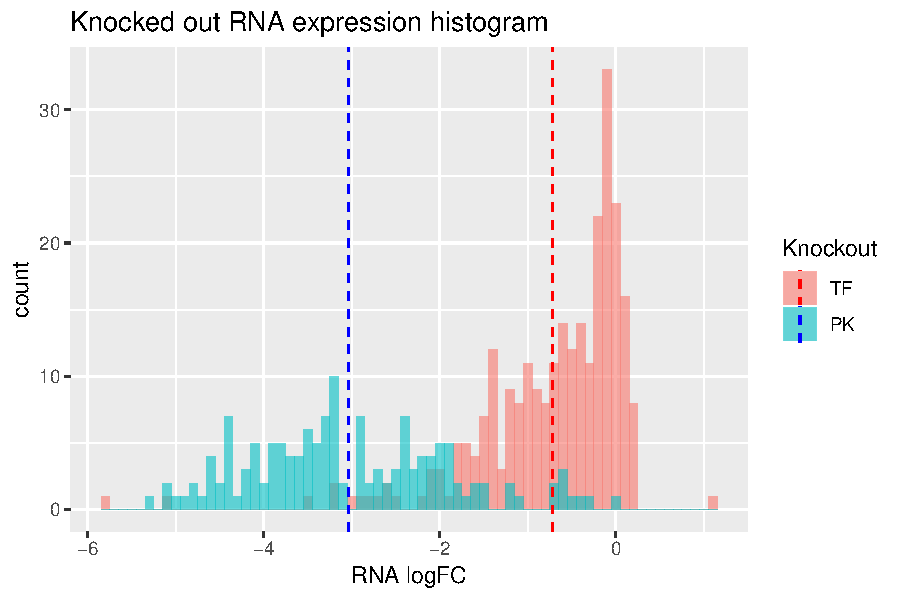
\includegraphics[width=\textwidth]{data/fig/knockout_RNA_hist.pdf}
  \caption{\textbf{KO RNA expression level histogram.} Subfig.~\ref{fig:KO_RNA_hist}. }
\end{figure}}
{\stepcounter{figure}}
\alt<2| handout:2>{
\begin{subequations}
\label{eq:discussion_linear}
\begin{align}
x_i &= \sum_j b_{ij} x_j
\\
\log \frac{x_i^{(ko)}}{x_i^{(wt)}} &=
\sum_j b_{ij} \log \frac{x_j^{(ko)}}{x_j^{(wt)}}
\\
\frac{x_i^{(ko)}}{x_i^{(wt)}} &=
\prod_j \left( \frac{x_j^{(ko)}}{x_j^{(wt)}} \right) ^{b_{ij}}
\end{align}
\end{subequations}}
{\stepcounter{equation}}
\alt<3| handout:3>{\begin{subequations}
\label{eq:prot_RNA}
\begin{align}
\dv{p_i}{t} &= m_i r_i - \lambda_i p_i
\\
\frac{p_i^{(ko)}}{p_i^{(wt)}} &= \frac{m_i r_i^{(ko)} - \dv{p_i^{(ko)}}{t}}{m_i r_i^{(wt)} - \dv{p_i^{(wt)}}{t}}
\end{align}
\end{subequations}
For $\dv{p_i^{(ko)}}{t} \rightarrow 0$ and $\dv{p_i^{(wt)}}{t} \rightarrow 0$ we then get
\begin{equation}
x_i =
\log \frac{p_i^{(ko)}}{p_i^{(wt)}} = \log
\frac{r_i^{(ko)}}{r_i^{(wt)}}
\end{equation}}
{\stepcounter{equation}}
\end{column}
\end{columns}
\end{frame}
